%   ####
%
%   Band VIII, 3 N.??A02 / ??X.2
%   Signatur/Tex-Datei: LH_37_01_020-021
%   RK-Nr. 38537 
%   Überschrift: [Omne quod sonat tremit]
%   Datierung: [zweite Hälfte August 1681 – 1682]
%   WZ: Blatt 20: RK-Wz 138 (insgesamt eins)
%.  SZ: (keins)
%.  Bilddateien (PDF): LH_37_01_020-021_d (insgesamt eine)
%
%
\begin{ledgroupsized}[r]{120mm}
\footnotesize%
\pstart%
\noindent%
\textbf{Überlieferung:}
\pend%
\end{ledgroupsized}
\begin{ledgroupsized}[r]{114mm}
\footnotesize%
\pstart%
\parindent -6mm
\makebox[6mm][l]{\textit{L}}%
Konzept: LH XXXVII 1 Bl. 20\textendash21.
Ein Bogen 2\textsuperscript{o};
ein Wasserzeichen auf Bl. 20.
Vier jeweils zum Falz hin einspaltig beschriebene Seiten.
% (Unsere Druckvorlage.)
\pend%
\end{ledgroupsized}
%
\begin{ledgroupsized}[r]{114mm}
\footnotesize%
\pstart%
\parindent -6mm
\makebox[6mm][l]{\textit{E}}%
\textsc{Gerland} 1906, S.~27\textendash31.\cite{00197}
\pend%
\end{ledgroupsized}
%
%
\vspace*{8mm}
%
%
\count\Bfootins=1000
\count\Afootins=1000
\count\Cfootins=1000
%
%
\pstart%
\normalsize%
\noindent%
%%%
\lbrack20~r\textsuperscript{o}\rbrack\ %%% Blatt 20r
%%%
Omne quod sonat tremit.
\pend%
%
\pstart%
Quicquid
\edtext{tremit aeri\protect\index{Sachverzeichnis}{aer} et corporibus}{%
\lemma{tremit}\Bfootnote{%
\textit{(1)}~corpori
\textit{(2)}~aeri et corporibus%
~\textit{L}}}
tensis\protect\index{Sachverzeichnis}{corpus tensum} sed maxime homotonis\protect\index{Sachverzeichnis}{corpus homotonum}
eandem trepidationem\protect\index{Sachverzeichnis}{trepidatio} communicat.
\pend%
%
\pstart%
%
Aures\protect\index{Sachverzeichnis}{auris} eo naturae artificio\protect\index{Sachverzeichnis}{artificium naturae} sunt conditae,
ut sint omnibus corporibus\protect\index{Sachverzeichnis}{corpus sonorum}
\edtext{\lbrack quorum\rbrack}{\lemma{quarum}\Bfootnote{\textit{L~ändert Hrsg.}}}
sonos\protect\index{Sachverzeichnis}{perceptio soni} percipimus homotonae.
\pend%
%
\pstart%
%
Auris corporum sonos\protect\index{Sachverzeichnis}{sonus} exprimit et imitatur.
\pend%
%
\pstart%
%
Objectum
\edtext{sonans\protect\index{Sachverzeichnis}{objectum sonans} est
instar chordae pulsatae,\protect\index{Sachverzeichnis}{chorda pulsata}
organon vero auditus\protect\index{Sachverzeichnis}{organon auditus} est instar chordae homotonae\protect\index{Sachverzeichnis}{chorda homotona}
sine tactu\protect\index{Sachverzeichnis}{tactus} resonantis.\protect\index{Sachverzeichnis}{chorda resonans}}{%
\lemma{sonans}\Bfootnote{% \hspace*{-0,5mm}
est instar chordae
\textit{(1)}~homotonae sine tactu resonantis
\textit{(2)}~pulsatae, organon \lbrack...\rbrack\ tactu resonantis.%
~\textit{L}}}
\pend%
%
\pstart%
%
\edtext{Tremere quid\lbrack:\rbrack\
itiones et reditiones\protect\index{Sachverzeichnis}{itio et reditio}
in chordis}{%
\lemma{Tremere}\Bfootnote{%
\textit{(1)}~quid est tensionem
\textit{(2)}~quid
\textit{(a)}~ch
\textit{(b)}~itiones et reditiones in chordis%
~\textit{L}}}
valde tensis\protect\index{Sachverzeichnis}{chorda tensa} fiunt ut in laxis,\protect\index{Sachverzeichnis}{chorda laxa}
\edtext{etsi non aeque oculis\protect\index{Sachverzeichnis}{oculus}
percipiantur.\protect\index{Sachverzeichnis}{perceptio ocularis}}{%
\lemma{etsi}\Bfootnote{%
\textit{(1)}~sint invisibiles
\textit{(2)}~non aeque oculis percipiantur.%
~\textit{L}}}
\pend%
%
\pstart%
%
\edtext{Quicquid tremit tensum est.}{%
\lemma{Quicquid}\Bfootnote{%
\hspace*{-0,5mm}tremit tensum est.\protect\index{Sachverzeichnis}{tensum}
\textit{erg.~L}}}
\pend%
%
\pstart%
%
Nullum corpus tam molle\protect\index{Sachverzeichnis}{corpus molle} est,
\edtext{quin celeri nimis}{%
\lemma{quin}\Bfootnote{%
\textit{(1)}~satis
\textit{(2)}~satis
\textit{(3)}~celeri nimis%
~\textit{L}}}
divisioni\protect\index{Sachverzeichnis}{divisio celeris} resistat.
 \pend%
%
\pstart%
%
\edtext{Quicquid\edlabel{LH_37_01_020r_culcitra-1}
divisioni resistit, id antequam rumpatur tenditur,
ut fila culcitrae.\protect\index{Sachverzeichnis}{filum}\protect\index{Sachverzeichnis}{culcitra}
\edlabel{LH_37_01_020r_culcitra-2}}{%
\lemma{Quicquid \lbrack...\rbrack\ culcitrae}\Cfootnote{%
Siehe den Ein\-wand in G.\,C. \textsc{Schelhammer}, Brief an G.\,W. Leibniz vom 13. (23.) April 1681 (\textit{LSB} III,~3 N.~206, S.~395.13\textendash396.5\cite{01200}).
Leibniz erwiderte hierauf zunächst in Rand\-bemer\-kun\-gen zu diesem Brief (ebd. S.~396, Anm. 11 u. 12)\cite{01200}
sowie in seiner Antwort vom 13. (23.) Januar 1682 (\textit{LSB} III,~3 N.~311, S.~545.10\textendash20; 550.8\textendash10).
Anspielungen auf Schelhammers Einwand finden sich zudem in
N.~12\textsubscript{1} (S.~\refpassage{LH_37_01_018r_Schelh-1}{LH_37_01_018r_Schelh-2})
% , N.~??X\textsubscript{3}, L1 (S.~\refpassage{LH_37_01_001r_culcitra-1}{LH_37_01_001r_culcitra-2})
und N.~12\textsubscript{3} (S.~\refpassage{LH_37_01_004r_culcitra-1}{LH_37_01_004r_culcitra-2}).}}
\pend%
%
\pstart%
%
Corporum repercussio\protect\index{Sachverzeichnis}{repercussio} omnis est
a restitutione tensorum\protect\index{Sachverzeichnis}{restitutio tensi}
et flexorum.\protect\index{Sachverzeichnis}{restitutio flexi}
Itaque quicquid repercutit tensum est.\protect\index{Sachverzeichnis}{tensum}
\pend%
%
\pstart%
%
Visibile hoc in pila\protect\index{Sachverzeichnis}{pila inflata}
\edtext{\lbrack inflata\rbrack,}{%
\lemma{inflato}\Bfootnote{\textit{erg.~L, ändert Hrsg.}}}
in pectine,\protect\index{Sachverzeichnis}{pecten} vel simili labente.
\pend%
%
\pstart%
%
Nihil tam durum quin nonnihil flectatur.\protect\index{Sachverzeichnis}{durum}
\pend%
\newpage
\pstart%
%
Nihil tam magnum quin nonnihil tremat.
\pend%
%
\pstart%
%
Ratio cur flexa\protect\index{Sachverzeichnis}{flexum}
et restituta\protect\index{Sachverzeichnis}{restitutum}
sponte iterum flectantur.
\pend%
%
\pstart%
%
Omne
\edtext{corpus cui}{%
\lemma{corpus}\Bfootnote{%
\textit{(1)}~quod
\textit{(2)}~cui%
~\textit{L}}}
continue novus impetus\protect\index{Sachverzeichnis}{impetus novus} imprimitur\lbrack,\rbrack\
novissime impetum habet ex omnibus collectum.\protect\index{Sachverzeichnis}{impetus collectus}
\pend%
%
\pstart%
%
Quicquid magnum impetum collegit,\protect\index{Sachverzeichnis}{impetus collectus}
id trans locum ubi alias quieturum esset feretur.%
\edtext{}{\lemma{\textit{\hspace{2mm}Am Rand:}}\Afootnote{Aqua\protect\index{Sachverzeichnis}{sonus aquae} et aer\protect\index{Sachverzeichnis}{sonus aeris} sonum edunt sola suarum partium collisione,\protect\index{Sachverzeichnis}{collisio partium} experimentum.\vspace{1em}\protect\index{Sachverzeichnis}{experimentum}}}%
\pend%
%
\pstart%
%
Non potest
\edtext{dici an et quando}{%
\lemma{dici}\Bfootnote{%
\textit{(1)}~quando
\textit{(2)}~an et quando%
~\textit{L}}}
cesset trepidatio\protect\index{Sachverzeichnis}{trepidatio}
tensi\protect\index{Sachverzeichnis}{tensum} semel
\edtext{pulsati.%
\edtext{}{\lemma{\textit{\hspace{2mm}Am Rand:}}\Afootnote{*\vspace{1em}}}%
%
\newline\indent%
%
Aer\protect\index{Sachverzeichnis}{aer}}{%
\lemma{pulsati.}\Bfootnote{%
\textit{(1)}~Aeris definitio
\textit{(2)}~Aer%
~\textit{L}}}
est fluidum elasticum.\protect\index{Sachverzeichnis}{fluidum elasticum}
\pend%
%
\pstart%
%
Et spiritus vini\protect\index{Sachverzeichnis}{spiritus vini}
esse videtur fluidum\protect\index{Sachverzeichnis}{fluidum elasticum}
aeri valde cognatum.
\pend%
%
\pstart%
%
Aqua\protect\index{Sachverzeichnis}{aqua} non est corpus satis elasticum,\protect\index{Sachverzeichnis}{corpus elasticum}
\edtext{(\phantom)\hspace*{-1.2mm}tractatus\protect\index{Sachverzeichnis}{tractatus}}{%
\lemma{tractatus}\Cfootnote{% \lbrack...\rbrack\ \textit{compressione}
\textsc{R.~Magiotti}, \textit{Renitenza certissima dell'acqua alla compressione}, Rom 1648.\cite{01196}}} % Möglicherweise zitiert nach \cite{}H.~\textsc{Fabri}, \textit{Physica}, tract. ??, lib. ??, prop. ?? 
\textit{della renitenza dell'acqua alla compressione}\lbrack\phantom(\hspace*{-1.2mm})\rbrack.%
\pend%
%
\pstart%
%
Circulus qui in aqua fit\protect\index{Sachverzeichnis}{circulus aqueus}
injecto lapillo,\protect\index{Sachverzeichnis}{lapillus injectus}
nihil est aliud quam fluctus orbicularis.\protect\index{Sachverzeichnis}{fluctus orbicularis}
\pend%
%
\pstart%
%
Ut ex uno fluctu nascitur alius
\edtext{parallelus}{\lemma{parallelus}\Bfootnote{\textit{erg.~L}}}
sed humilior,
ita ex fluctu orbiculari nascitur alius orbicularis remotior,
ac proinde major priore; sed
\edtext{humilior.\protect\index{Sachverzeichnis}{fluctus orbicularis}
%
\newline\indent%
%
Fluctus aquae\protect\index{Sachverzeichnis}{fluctus aquae} potius conferendi sunt}{%
\lemma{humilior.}\Bfootnote{%
\textit{(1)}~Fluctuum aquae propagatio,\protect\index{Sachverzeichnis}{propagatio fluctuum}
\textit{(a)}~nihil commune h
\textit{(b)}~tantum differt
\textit{(c)}~potius conferenda est
\textit{(2)}~Fluctus aquae potius conferendi sunt%
~\textit{L}}}
vento\protect\index{Sachverzeichnis}{ventus} in aere quam sono.\protect\index{Sachverzeichnis}{sonus}
\pend%
%
\pstart%
%
Sonus non oritur\protect\index{Sachverzeichnis}{origo soni}
ex percussione\protect\index{Sachverzeichnis}{percussio}
corporis sonantis\protect\index{Sachverzeichnis}{corpus sonans} immediate,
sed ex restitutione\protect\index{Sachverzeichnis}{restitutio percussi}
\edtext{percussi.
\newline\indent%
%
\edtext{}{\lemma{\textit{Am Rand:}}\Afootnote{*\vspace{-4mm}}}%
Ad sonum}{%
\lemma{percussi}\Bfootnote{%
\hspace*{-0,5mm}\textbar~eaque non una sed pluribus repetitis \textit{gestr.}~%
\textbar~. Ad sonum%
~\textit{L}}}
sensibilem\protect\index{Sachverzeichnis}{sonus sensibilis} efficiendum
opus est multis trepidationibus repetitis\protect\index{Sachverzeichnis}{trepidatio repetita}%
\textso{ ut ad videndum aliquod punctum sensibile,}\protect\index{Sachverzeichnis}{punctum sensibile}%
\textso{ multis est opus radiis.}\protect\index{Sachverzeichnis}{radius}%
\textso{ Ita ad videndum apicem montis,}\protect\index{Sachverzeichnis}{apex montis}%
\textso{ qui instar puncti videtur.}
%%%
\lbrack20~v\textsuperscript{o}\rbrack%%% Blatt 20v
\pend
\pstart
Si aer\protect\index{Sachverzeichnis}{aer percussus} subito
\edtext{percutiatur, pars ejus\protect\index{Sachverzeichnis}{pars aeris}
quae est ante rem \lbrack percutientem\rbrack\ comprimitur,\protect\index{Sachverzeichnis}{aer compressus}}{%
\lemma{percutiatur,}\Bfootnote{%
\textit{(1)}~ante
\textit{(2)}~\textbar~is qui \textit{streicht Hrsg.}~\textbar\
\textit{(3)}~pars ejus quae est ante rem
\textbar~percussam \textit{ändert Hrsg.}
\textbar~percussam \textit{streicht Hrsg.}~%
\textbar\ comprimitur,%
~\textit{L}}}
%
\makebox[1.0\textwidth][s]{pars quae post eam est rarescit.\protect\index{Sachverzeichnis}{aer rarefactus}
\edtext{Sit corpus $AB$}{%
\lemma{Sit}\Bfootnote{%
\textit{(1)}~aer
\textit{(2)}~corpus $AB$%
~\textit{L}}}
\edtext{\lbrack quod\rbrack}{%
\lemma{quo}\Bfootnote{\textit{L~ändert Hrsg.}}}
%
magna celeritate\protect\index{Sachverzeichnis}{celeritas percussionis} transfertur in}
%%%
\pend%
%
  \newpage% PR: Rein vorläufig !!!!
 % \vspace*{-0.5em}
  \centerline{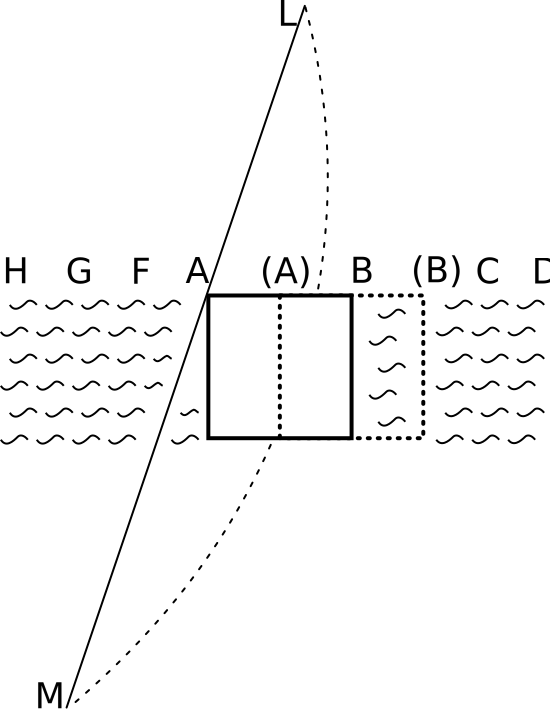
\includegraphics[width=0.42\textwidth]{gesamttex/edit_VIII,3/images/LH_37_01_020-021_d.pdf}}%\\
  \vspace{0.5em}
  \centerline{\lbrack\textit{Fig.~1}\rbrack}%
  \label{LH_37_01_020-021_fig.1}%
  \vspace{2.0em}
%  \newpage% PR: Rein vorläufig !!!!
%
\pstart%
%
\noindent \edtext{}{\lemma{\hspace*{1,6mm}\lbrack\textit{Fig.~1}\rbrack}\killnumber\Cfootnote{%
In einer ersten, verworfenen und daher nicht wiedergegebenen Fassung des Diagramms verläuft die Saite $LM$ schräg durch den Körper $AB$ hindurch.}}%
% ACHTUNG !!! D diese C-footnote hängt nicht mit dem Text, sondern mit der Abbildung [Fig.~1] zusammen !!!
\textit{(A)(B)}, et percutiet
\edtext{aerem\protect\index{Sachverzeichnis}{aer percussus} $L$ anteriorem}{%
\lemma{aerem}\Bfootnote{%
\hspace*{-0,5mm}\textbar~$L$ \textit{erg.}~%
\textbar\ anteriorem%
~\textit{L}}}
\edtext{\lbrack$BC$\rbrack,}{\lemma{$BE$}\Bfootnote{\textit{L~ändert Hrsg.}}}
eumque expellet\protect\index{Sachverzeichnis}{aer expulsus} ex loco \textit{B(B)}.
Et quoniam aer tanta celeritate\protect\index{Sachverzeichnis}{celeritas aeris}
circulum\protect\index{Sachverzeichnis}{circulus aeris} commode peragere non potest,
ut statim tantundem
\edtext{aeris, eundem quam ante densitatis gradum\protect\index{Sachverzeichnis}{gradus densitatis}}{%
\lemma{aeris,}\Bfootnote{%
\textit{(1)}~eandem quam ante rarita
\textit{(2)}~eundem quam ante
\textit{(a)}~compressionis
\textit{(b)}~densitatis gradum%
~\textit{L}}}
habentis expellatur
\edtext{ex \lbrack$BC$\rbrack, et vicissim
% \edlabel{LH37,01_20v_ref-01}%
% \edtext{}{{\xxref{LH37,01_20v_ref-01}{LH37,01_20v_ref-02}}\lemma{succedat in}\Bfootnote{%
% \textbar~succedat in \textit{streicht Hrsg.}~\textbar\ locum~\textit{L}}}%
succedat in}{%
\lemma{ex}\Bfootnote{% \hspace*{-0,5mm}
\textbar~\textit{(B)E} \textit{ändert Hrsg.}~\textbar\ 
\textit{(1)}~\textbar~succedat in \textit{streicht Hrsg.}~\textbar\ 
\textit{(2)}~et vicissim succedat in%
~\textit{L}}}
% \edlabel{LH37,01_20v_ref-02}
locum ipsius $FA$ succedentis in locum\protect\index{Sachverzeichnis}{locus relictus} a corpore relictum $AB,$
quia corpora elastica\protect\index{Sachverzeichnis}{corpus elasticum} malunt tendi
\edtext{nonnihil}{\lemma{nonnihil}\Bfootnote{\textit{erg.~L}}}
quam celeriter moveri;
hinc necesse
\edtext{est aere \textit{B(B)} expulso\protect\index{Sachverzeichnis}{aer expulsus}
a corpore $AB$ et in locum ipsius
\lbrack \textit{(B)C}\rbrack\
non satis statim recedentis subeunte,}{%
\lemma{est}\Bfootnote{%
\textit{(1)}~aerem \textit{B(B)} subeun
\textit{(2)}~aere \textit{B(B)} \lbrack...\rbrack\ locum ipsius
\textbar~\textit{(B)E} \textit{ändert Hrsg.}~%
\textbar\ non satis statim recedentis subeunte,%
~\textit{L}}}
aerem in loco
\edtext{\lbrack\textit{(B)C}\rbrack}{%
\lemma{\textit{(B)(E)}}\Bfootnote{\textit{L~ändert Hrsg.}}}
% \edtext{loco \lbrack\textit{(B)C}\rbrack\ existentem}{%
% \lemma{loco}\Bfootnote{%
% \hspace*{-0,5mm}\textbar~\textit{(B)(E)} \textit{ändert Hrsg.}~%
% \textbar\ existentem~%
% \textit{L}}}
existentem nonnihil comprimi\protect\index{Sachverzeichnis}{aer compressus} et in loco $FA$ existentem,
quia etiam locum
\edtext{\lbrack\textit{A(A)}\rbrack}{%
\lemma{$AC$}\Bfootnote{\textit{L~ändert Hrsg.}}}
a corpore
\edtext{$AB$ desertum\protect\index{Sachverzeichnis}{locus desertus}}{%
\lemma{$AB$}\Bfootnote{%
\textit{(1)}~repletu
\textit{(2)}~desertum%
~\textit{L}}}
implere debet,
\edtext{novo aere\protect\index{Sachverzeichnis}{aer novus} sufficiente}{%
\lemma{novo}\Bfootnote{%
\textit{(1)}~corpore su
\textit{(2)}~aere sufficiente%
~\textit{L}}}
non statim succedente dilatari.\protect\index{Sachverzeichnis}{aer dilatatus}%
\pend%
%
%
\newpage
\pstart%
Si in medio aere ordinario\protect\index{Sachverzeichnis}{aer ordinarius}
\edtext{sit locus\protect\index{Sachverzeichnis}{locus repletus} repletus}{%
\lemma{sit}\Bfootnote{%
\textit{(1)}~pars
\textit{(2)}~locus
\textbar~repletus \textit{erg.}~\textbar%
~\textit{L}}}
%
aere justo dilatatiori,\protect\index{Sachverzeichnis}{aer dilatatus}
aer circumstans\protect\index{Sachverzeichnis}{aer circumstans}
magno impetu\protect\index{Sachverzeichnis}{impetus aeris} in eum irruens
jam tum aliquem efficiet sonum.\protect\index{Sachverzeichnis}{sonus}
\edtext{Experimentum\protect\index{Sachverzeichnis}{experimentum} est in Machinis Gerickianis;\protect\index{Sachverzeichnis}{machina Gerickiana}
nam si duo hemisphaeria\protect\index{Sachverzeichnis}{hemisphaerium Gerickianum}
ex quibus exhaustus est aer,\protect\index{Sachverzeichnis}{aer exhaustus} divellantur,
aer circumstans\protect\index{Sachverzeichnis}{aer circumstans} ad locum replendum\protect\index{Sachverzeichnis}{locus replendus} confluens
sonum edit instar sclopeti.\protect\index{Sachverzeichnis}{sonus sclopeti}}{%
\lemma{Experimentum \lbrack...\rbrack\ sclopeti}\Cfootnote{%
Siehe \textsc{O.\,v.\,Guericke}, \textit{Experimenta nova}, lib. III, cap. 25 (Amsterdam 1672, S.~106\,f.)\cite{00055}
Die von Leibniz erwähnten \textit{Machinae Gerickianae} sind Instrumente zur Vakuum\-erzeugung,
die Guericke entwickelt und im dritten Buch seiner \textit{Experimenta nova} beschrieben hatte.
Leibniz hat hieraus Auszüge verfasst (\textit{LSB} VIII,~1 N.~36).\cite{01197}}}
\pend%
%
% \newpage% REIN VORLÄUFIG
\pstart%
\edtext{Idem proportione continget in loco}{%
\lemma{Idem}\Bfootnote{%
\textit{(1)}~continget et in nostro
\textit{(2)}~proportione continget in loco%
~\textit{L}}}
$FA.$
Etsi enim exigua
\edtext{sit aeris in eo dilatatio,\protect\index{Sachverzeichnis}{dilatatio aeris}}{%
\lemma{sit}\Bfootnote{%
\textit{(1)}~differentia ejus
\textit{(2)}~aeris in eo dilatatio,%
~\textit{L}}}
et exiguus etiam ipse
\edtext{locus,
(\phantom)\hspace*{-1.2mm}%
tantus scilicet \lbrack quanto\rbrack\ chorda tremens\protect\index{Sachverzeichnis}{chorda tremens}
major apparet se quiescente%
\phantom(\hspace*{-1.2mm})}{%
\lemma{locus,}\Bfootnote{%
\textit{(1)}~invisibilis scilicet
\textit{(2)}~(\phantom)\hspace*{-1.2mm}tantus scilicet \textbar~quando \textit{ändert Hrsg.}~\textbar\ chorda tremens major apparet
\textit{(a)}~dimidio sui quiescentis
\textit{(b)}~se quiescente\phantom(\hspace*{-1.2mm})%
~\textit{L}}}
orietur tamen si non sonus\protect\index{Sachverzeichnis}{origo soni}
certe soni rudimentum,\protect\index{Sachverzeichnis}{rudimentum soni}
id est, quod percipi possit multis repetitionibus.%
\protect\index{Sachverzeichnis}{repetitio soni}\protect\index{Sachverzeichnis}{perceptio soni}
\pend%
%
\pstart%
Ex \edtext{aere ambiente,\protect\index{Sachverzeichnis}{aer ambiens} dum}{%
\lemma{aere}\Bfootnote{%
\textit{(1)}~iterum confluente
\textit{(2)}~ambiente,
\textit{(a)}~novum
\textit{(b)}~dum%
~\textit{L}}}
scilicet locus $FA$
\edtext{aeris dilatati\protect\index{Sachverzeichnis}{aer dilatatus}}{%
\lemma{aeris}\Bfootnote{% \hspace*{-0,5mm}
dilatati \textit{erg.~L}}}
iterum
\edtext{impletur, in locum $FA$ cum impetu\protect\index{Sachverzeichnis}{impetus aeris} ex $GF$ confluente,}{%
\lemma{impletur,}\Bfootnote{%
\textit{(1)}~et locus $BC$ depletur, cum impetu confluente,
\textit{(2)}~in locum \lbrack...\rbrack\ $GF$ confluente,%
~\textit{L}}}
\edtext{et ex aere compresso\protect\index{Sachverzeichnis}{aer compressus} incluso in loco \textit{(B)C}
dum is depletur et in vicinum aerem\protect\index{Sachverzeichnis}{aer vicinus} $CD$ erumpit,}{%
\lemma{et}\Bfootnote{%
\hspace*{-0,5mm}ex aere
\textit{(1)}~incluso dum
\textit{(2)}~compresso incluso \lbrack...\rbrack\ $CD$ erumpit,
\textit{erg.~L}}}
nova oritur percussio,\protect\index{Sachverzeichnis}{percussio aeris}
novaque iterum compressio\protect\index{Sachverzeichnis}{compressio aeris} et dilatatio.\protect\index{Sachverzeichnis}{dilatatio aeris}
\pend%
%
\pstart%
Dum aer vicinus\protect\index{Sachverzeichnis}{aer vicinus}
\edtext{$GF$}{\lemma{$GF$}\Bfootnote{\textit{erg.~L}}}
irruit in locum\protect\index{Sachverzeichnis}{locus replendus}
\edtext{replendum $FA,$ ipse}{%
\lemma{replendum}\Bfootnote{%
\hspace*{-0,5mm}\textbar~%
\textit{(1)}~aut excipit aerem deplendum ex loco deplendo $BC$
\textit{(2)}~$FA$
\textit{erg.}~%
\textbar~, ipse%
~\textit{L}}}
quoque nonnihil
\edtext{dilatatur,\protect\index{Sachverzeichnis}{aer dilatatus} ubi cohaeret aeri $GH$; a quo}{%
\lemma{dilatatur,}\Bfootnote{%
\textit{(1)}~nam subito divellitur ab eo cui
\textbar~remotiori \textit{erg.}~%
\textbar\ antea cohaerebat, vel etiam sub
\textit{(2)}~nam
\textit{(3)}~ubi cohaeret aeri $GH$;
\textit{(a)}~a quo
\textit{(b)}~a quo%
~\textit{L}}}
satis celeriter sine dilatatione aliqua divelli non potest.
Et quemadmodum dilatatio\protect\index{Sachverzeichnis}{dilatatio aeris} ex $FA$ propagatur in $GF,$
ita ex $GF$ propagatur in $HG.$
\pend%
% \newpage% % % %   REIN VORLÄUFIG   ! ! ! ! 
%
\pstart%
Similiter compressio\protect\index{Sachverzeichnis}{compressio aeris} propagatur,
dum enim locus
\edtext{\textit{(B)C} nonnihil}{%
\lemma{\textit{(B)C}}\Bfootnote{%
\hspace*{-0,5mm}\textbar~in quo \textit{erg.~L, streicht Hrsg.}~%
\textbar\ nonnihil%
~\textit{L}}}
compressus\protect\index{Sachverzeichnis}{locus compressus} subito depletur in locum $CD,$
necesse est $CD$ nonnihil comprimi;
similiterque ex $CD$ compressio\protect\index{Sachverzeichnis}{compressio aeris} porro in sequentem adhuc remotiorem propagatur.
\pend%
\pstart%
Omnem autem compressionem\protect\index{Sachverzeichnis}{compressio aeris} sequitur mox
\edtext{restitutio dilatans,\protect\index{Sachverzeichnis}{restitutio dilatans}}{%
\lemma{restitutio}\Bfootnote{%
\textit{(1)}~dil
\textit{(2)}~iterum
\textit{(3)}~dilatans,%
~\textit{L}}}
et dilatationem\protect\index{Sachverzeichnis}{dilatatio aeris} restitutio iterum comprimens;\protect\index{Sachverzeichnis}{restitutio comprimens}
ita aer jam ipse per se aliquamdiu in vibrationes\protect\index{Sachverzeichnis}{vibratio aeris} peraget,
etsi corpus sonans\protect\index{Sachverzeichnis}{corpus sonans} non vibraret.
Sed non erit satis sensibilis illa vibratio,\protect\index{Sachverzeichnis}{vibratio sensibilis}
quia ex una tantum percussione\protect\index{Sachverzeichnis}{percussio aeris} orta est corporis $AB$ semel tantum translati in \textit{(A)(B)}.
%%%
\lbrack21~r\textsuperscript{o}\rbrack%%% Blatt 21r
%%%
\pend%
%
\newpage% REIN VORLÄUFIG
\pstart%
Si corpus\protect\index{Sachverzeichnis}{corpus tremens}
\edtext{tremens vel ejus pars}{%
\lemma{tremens}\Bfootnote{%
\hspace*{-0,5mm}vel ejus pars
\textit{erg.~L}}}
$AB$ translatum in \textit{(A)(B)} redeat in $AB,$
et iterum
\edtext{\lbrack in\rbrack}{\lemma{in}\Bfootnote{\textit{erg. Hrsg.}}}
\textit{(A)(B)} aliquoties reciprocatis itionibus et reditionibus,\protect\index{Sachverzeichnis}{itio et reditio}
\edtext{toties aer denuo percutietur,\protect\index{Sachverzeichnis}{aer percussus}
et novum impetum\protect\index{Sachverzeichnis}{impetus aeris} acquiret,}{%
\lemma{toties}\Bfootnote{%
\textit{(1)}~, novum impetum imprimet aer
\textit{(2)}~aer denuo \lbrack...\rbrack\ impetum acquiret,%
~\textit{L}}}
qui denique tam fortis fiet, ut possit percipi.\protect\index{Sachverzeichnis}{perceptio soni}
\pend%
% \newpage%     REIN VORLÄUFIG
%
\pstart%
\edtext{Praeterea si vibrationes\protect\index{Sachverzeichnis}{vibratio aeris}}{%
\lemma{Praeterea}\Bfootnote{%
\textit{(1)}~cum vibrationes
\textit{(2)}~si vibrationes%
~\textit{L}}}
aeris a dilatatione\protect\index{Sachverzeichnis}{dilatatio aeris}
ad compressionem\protect\index{Sachverzeichnis}{compressio aeris} reciproce transeuntis
\edtext{non sint synchronae\protect\index{Sachverzeichnis}{vibratio synchrona}}{%
\lemma{non}\Bfootnote{%
\textit{(1)}~consentia
\textit{(2)}~sint
\textit{(a)}~unisonae
\textit{(b)}~synchronae%
~\textit{L}}}
reciprocationibus\protect\index{Sachverzeichnis}{reciprocatio corporis trementis}
corporis\protect\index{Sachverzeichnis}{corpus tremens} trementis\lbrack,\rbrack\
tunc novae supervenientes\protect\index{Sachverzeichnis}{percussio superveniens}
\edtext{percussiones aerique impressae impetus}{%
\lemma{percussiones}\Bfootnote{%
\textit{(1)}~impetus
\textit{(2)}~aerique impressae impetus%
~\textit{L}}}
reciprocandi\protect\index{Sachverzeichnis}{impetus reciprocandi}
quos aer ex priore adhuc percussione\protect\index{Sachverzeichnis}{percussio prior} residuos habet
turbabunt; nam
\edtext{aliquando}{\lemma{aliquando}\Bfootnote{\textit{erg.~L}}}
dilatandi\protect\index{Sachverzeichnis}{impetus dilatandi}
\edtext{sese}{\lemma{sese}\Bfootnote{\textit{erg.~L}}}
impetum imprement aeri dum ipse
\edtext{jam}{\lemma{jam}\Bfootnote{\textit{erg.~L}}}
tendit ad compressionem;\protect\index{Sachverzeichnis}{compressio aeris} aut contra.
Videndum igitur qua arte efficiat natura,\protect\index{Sachverzeichnis}{ars naturae}
ut perturbatio\protect\index{Sachverzeichnis}{perturbatio} ista
\edtext{evitetur.%
\newline\indent%
%
Si duo corpora\protect\index{Sachverzeichnis}{corpus tensum} inaequalia sint}{%
\lemma{evitetur.}\Bfootnote{%
\textit{(1)}~Omne corpus
\textit{(2)}~Si duo corpora
\textit{(a)}~sint
\textit{(b)}~inaequalia sint%
~\textit{L}}}
ejusdem \protect\index{Sachverzeichnis}{tensio}tensionis\lbrack,\rbrack\
percussum\protect\index{Sachverzeichnis}{corpus percussum}
%
\edtext{eo celeriores habet reciprocationes,\protect\index{Sachverzeichnis}{reciprocatio corporis percussi}
quo est minus.
\edlabel{LH_37_01_021r_uwdci-1}%
Hujus propositionis\protect\index{Sachverzeichnis}{propositio} veram rationem}{%
\lemma{eo}\Bfootnote{%
\textit{(1)}~celerius restituitur
\textit{(2)}~celeriores habet \lbrack...\rbrack\ est minus. % reciprocationes, quo
\textit{(a)}~Hanc
\textit{(b)}~Hujus propositionis
\textit{(aa)}~veras rationes
\textit{(bb)}~veram rationem%
~\textit{L}}}
%
aliquando reddam.\edlabel{LH_37_01_021r_uwdci-2}%
\edtext{}{%
{\xxref{LH_37_01_021r_uwdci-1}{LH_37_01_021r_uwdci-2}}%
{\lemma{Hujus \lbrack...\rbrack\ reddam}\Cfootnote{%
Dieses Gesetz hatte Leibniz (mit Bezug auf Saiten) bereits im Dezember 1680 dargelegt und begründet;
siehe N.~\ref{41152_2}, %??A10,
S.~\refpassage{LH_35_09_15_009v_utlong-1}{LH_35_09_15_009v_utlong-2};
N.~\ref{41153}, %??A11,
S.~\refpassage{LH_35_09_15_005r_quominoreocitius-1}{LH_35_09_15_005r_quominoreocitius-2}.%
}}}
%
Nunc satis est eam assumere velut comprobatam experimento.\protect\index{Sachverzeichnis}{experimentum}
Nam
\edtext{constat ex sectione monochordi\protect\index{Sachverzeichnis}{sectio monochordi}
\edlabel{LH_37_01_021r_freqzulaeng-1}chordam\protect\index{Sachverzeichnis}{chorda tensa} quo est minor,
eo sonum reddere acutiorem\protect\index{Sachverzeichnis}{sonus acutus} manente eadem
\edtext{tensione;\edlabel{LH_37_01_021r_freqzulaeng-2}\protect\index{Sachverzeichnis}{tensio chordae} idem}{%
\lemma{tensione;}\Bfootnote{%
\textit{(1)}~item
\textit{(2)}~idem%
~\textit{L}}}
de corporibus quoque alterius figurae\protect\index{Sachverzeichnis}{figura corporis} constat.}{%
\lemma{constat \lbrack...\rbrack\ constat}\Cfootnote{%
Siehe etwa \cite{01205}\textsc{Mersenne}, \textit{Harmonie universelle}, livre III des mouvemens, prop. 5 [6]; 8 [9] (Bd.~I, S.~A, 169; 174\,f.); livre III des instrumens, prop. 7\textendash9 (Bd.~II, S.~D, 123\textendash128).}}
\pend%
%
\count\Bfootins=1000
\count\Afootins=1000
\count\Cfootins=1000
\pstart%
Consideremus jam quanta esse debeat
portio aeris\protect\index{Sachverzeichnis}{portio aeris} $AF,$ $FG,$ item \textit{(B)C}, aut
\edtext{$CD,$ et utique apparet hoc esse satis}{%
\lemma{$CD,$}\Bfootnote{%
\textit{(1)}~satis
\textit{(2)}~et utique apparet hoc esse satis%
~\textit{L}}}
indeterminatum; et primis ictibus,\protect\index{Sachverzeichnis}{ictus primus}
\edtext{ut portiones aeris\protect\index{Sachverzeichnis}{portio aeris} majores minoresve}{%
\lemma{ut}\Bfootnote{%
\textit{(1)}~modo haec modo illae p
\textit{(2)}~portiones aeris majores minoresve%
~\textit{L}}}
eligantur, ex variis pendere posse casibus,\protect\index{Sachverzeichnis}{casus}
prout ipsum corpus $AB$ non tantum majus minusve est,
sed et plures habet cavernas,\protect\index{Sachverzeichnis}{caverna} quibus
\edtext{aer ipsum ingreditur,\protect\index{Sachverzeichnis}{aer ingressus}}{%
\lemma{aer}\Bfootnote{%
\textit{(1)}~inclusus\protect\index{Sachverzeichnis}{aer inclusus}
\textit{(2)}~ipsum
\textit{(a)}~aer
\textit{(b)}~ingreditur,%
~\textit{L}}}
eo enim velut totidem filis\protect\index{Sachverzeichnis}{filum}
aerem ambientem\protect\index{Sachverzeichnis}{aer ambiens} fortius
%
\edtext{}{{\xxref{KZeitz131}{KZeitz132}}%
{%
\lemma{trahet;}\Bfootnote{%
\textit{(1)}~quaeque
\textit{(2)}~ut taceam
\textit{(a)}~de u
\textit{(b)}~diversa corpora heterogenea%
~\textit{L}}}}
\edlabel{KZeitz131}trahet;
ut taceam diversa corpora \makebox[1.0\textwidth][s]{heterogenea\protect\index{Sachverzeichnis}{corpus heterogeneum}\edlabel{KZeitz132}
%
quae in
\edtext{aere in diversis portionibus\protect\index{Sachverzeichnis}{portio aeris} diversimode reperiuntur.}{%
\lemma{aere}\Bfootnote{%
\textit{(1)}~reperiuntur
\textit{(2)}~in diversis portionibus diversimode reperiuntur.%
~\textit{L}}}
Verum haec}
\pend
\newpage
\pstart
\noindent de primis ictibus\protect\index{Sachverzeichnis}{ictus primus} intelligenda
\edtext{sunt, at corpore sonoro\protect\index{Sachverzeichnis}{corpus sonorum}
suas reciprocationes\protect\index{Sachverzeichnis}{reciprocatio corporis sonori} continuante paulatim}{%
\lemma{sunt,}\Bfootnote{%
\textit{(1)}~verum
\textit{(2)}~at
\textit{(a)}~paulatim
\textit{(b)}~corpore sonoro \lbrack...\rbrack\ continuante paulatim%
~\textit{L}}}
aer ita se componit,
ut fiat unisonus\protect\index{Sachverzeichnis}{aer unisonus}
corpori sonoro,\protect\index{Sachverzeichnis}{corpus sonorum}
ut nempe vibrationum aeris\protect\index{Sachverzeichnis}{vibratio aeris}
et corporis sonori\protect\index{Sachverzeichnis}{vibratio corporis sonori}
sibi obstantium perturbatio\protect\index{Sachverzeichnis}{perturbatio}
minuatur;
atque ita tum cum ex repetitis percussionibus\protect\index{Sachverzeichnis}{percussio repetita}
acceptus ab aere impetus\protect\index{Sachverzeichnis}{impetus acceptus}
satis redditus est validus ut percipi possit,\protect\index{Sachverzeichnis}{perceptio soni}
jam aer etiam ad unisonum\protect\index{Sachverzeichnis}{unisonus} devenit;
\edtext{id est in portiones\protect\index{Sachverzeichnis}{portio aeris} discerptus est
$AF,$ $FG,$ $GH$ etc. \textit{(B)C}, $CD$ etc. tantae magnitudinis,\protect\index{Sachverzeichnis}{magnitudo portionis aeris}
quantae in data aeris tensione\protect\index{Sachverzeichnis}{tensio aeris} faciant,
ut vibrationes portionum aeris\protect\index{Sachverzeichnis}{vibratio portionis aeris}}{%
\lemma{id}\Bfootnote{%
\hspace{-0,5mm}est
\textit{(1)}~tanta ejus portio vib
\textit{(2)}~in portiones \lbrack...\rbrack\ ut vibrationes
\textit{(a)}~aeris
\textit{(b)}~portionum aeris%
~\textit{L}}}
cum vibrationibus sonori\protect\index{Sachverzeichnis}{vibratio corporis sonori}
sint aeque diuturnae.\protect\index{Sachverzeichnis}{vibratio aequidiuturna}
\pend%
%
\count\Bfootins=1000
\count\Afootins=1000
\count\Cfootins=1000
\pstart%
Nam
\edtext{aer suum habet determinatum Elastrum\protect\index{Sachverzeichnis}{elastrum aeris}
sive tensionem\protect\index{Sachverzeichnis}{tensio aeris}}{%
\lemma{aer}\Bfootnote{%
\textit{(1)}~suam habet determinatam tensi
\textit{(2)}~suum habet \lbrack...\rbrack\ sive tensionem%
~\textit{L}}}
(\phantom)\hspace*{-1.2mm}%
utor autem hic tensionis\protect\index{Sachverzeichnis}{tensio}
voce generaliter pro compressione\protect\index{Sachverzeichnis}{compressio}
vel dilatatione,\protect\index{Sachverzeichnis}{dilatatio}
vel etiam flexione\protect\index{Sachverzeichnis}{flexio}
quae fit sine utroque, aut cum utroque simul,
ut in arcu tenso\protect\index{Sachverzeichnis}{arcus tensus}%
\phantom(\hspace*{-1.2mm})
%%%
\lbrack21~v\textsuperscript{o}\rbrack\ %%% Blatt 21v
%%%
quae oritur ex pondere aeris\protect\index{Sachverzeichnis}{pondus aeris} superstantis.
Itaque eligitur
\edtext{magnitudo partium,\protect\index{Sachverzeichnis}{magnitudo partis aeris} quae cum}{%
\lemma{magnitudo}\Bfootnote{%
\textit{(1)}~quae cum
\textit{(2)}~partium, quae cum%
~\textit{L}}}
data
\edtext{tensione,\protect\index{Sachverzeichnis}{tensio aeris} diuturnitatis desideratae}{%
\lemma{tensione,}\Bfootnote{%
\textit{(1)}~datae
\textit{(2)}~diuturnitatis desideratae%
~\textit{L}}}
(\phantom)\hspace*{-1.2mm}%
quae scilicet sonori est%
\phantom(\hspace*{-1.2mm})
exhibeat vibrationem.\protect\index{Sachverzeichnis}{vibratio partis aeris}
\pend%
%
\pstart%
Itaque in locis altioribus\protect\index{Sachverzeichnis}{locus altus} ut
\edtext{montibus,\protect\index{Sachverzeichnis}{mons} majoribus opus est}{%
\lemma{montibus,}\Bfootnote{%
\textit{(1)}~major eligetur
\textit{(2)}~majoribus opus est%
~\textit{L}}}
partibus aeris,\protect\index{Sachverzeichnis}{pars aeris}
quae causa esse potest cur sonus illic sit debilior.\protect\index{Sachverzeichnis}{sonus debilis}
Nam in majoribus portionibus\protect\index{Sachverzeichnis}{portio aeris} non tam exacte res succedit
ut in minoribus, ob varia impedimenta;\protect\index{Sachverzeichnis}{impedimentum}
\edtext{et cum aer}{%
\lemma{et}\Bfootnote{%
\textit{(1)}~aer cu
\textit{(2)}~cum aer%
~\textit{L}}}
ibi sit valde\protect\index{Sachverzeichnis}{aer rarus}
\edtext{rarus respectu puri}{%
\lemma{rarus}\Bfootnote{%
\textit{(1)}~quatenus pur
\textit{(2)}~respectu puri%
~\textit{L}}}
aeris,\protect\index{Sachverzeichnis}{aer purus} est tamen non ideo minus heterogeneis partibus\protect\index{Sachverzeichnis}{pars aeris heterogenea}
\edtext{plenus; quae}{%
\lemma{plenus;}\Bfootnote{%
\textit{(1)}~itaque
\textit{(2)}~quae%
~\textit{L}}}
servire poterunt ad
\edtext{explicandam causam\protect\index{Sachverzeichnis}{causa}
cur sclopeti sonus\protect\index{Sachverzeichnis}{sonus sclopeti} solito exilior fuerit in
Carpathii\protect\index{Ortsregister}{Karpaten (Mons Carpathius)}
cujusdam montis apice,\protect\index{Sachverzeichnis}{apex montis}
\edtext{quod Frolichius\protect\index{Namensregister}{\textso{Fr{\"o}lich} (Frolichius, Frölichius), David 1595\textendash1648}
sibi evenisse narrat.}{%
\lemma{quod \lbrack...\rbrack\ narrat}\Cfootnote{%
\textsc{D.\,Frölich}, \textit{Cynosura peregrinantium}, Ulm 1643, S.~268\textendash288.\cite{00047} % Bibliotheca sive 
Auch \textsc{Guericke}, \textit{Experimenta nova}, lib. V, cap. 8 (S.~162) berichtet über Frölichs Erzählung.\cite{00055}
Leibniz hat Guerickes Referat exzerpiert (\textit{LSB} VIII,~1 N.~36, S.~266.5\textendash7.\cite{01197})}}%
}{\lemma{explicandam}\Bfootnote{%
\textit{(1)}~narrationem quam habet
\textit{(2)}~causam
\textit{(a)}~eorum
\textit{(b)}~ejus quod Frolichius\protect\index{Namensregister}{\textso{Fr{\"o}lich} (Frolichius, Frölichius), David 1595\textendash1648}
in Carpathii\protect\index{Ortsregister}{Karpaten (Mons Carpathius)} cujusdam montis apice sibi evenisse narrat
\textit{(c)}~cur sclopeti \lbrack...\rbrack\ evenisse narrat.%
~\textit{L}}}
% \pend%
%\newpage% 
%
% \pstart%
Etiam
\edtext{in vacuo Gerickiano\protect\index{Sachverzeichnis}{vacuum Gerickianum} sonus\protect\index{Sachverzeichnis}{sonus in vacuo}}{%
\lemma{in}\Bfootnote{%
\textit{(1)}~vacuo sonus
\textit{(2)}~vacuo Gerickiano sonus%
~\textit{L}}}
admodum debilitatur, ipso
\edtext{Gerickio\protect\index{Namensregister}{\textso{Guericke} (Gerickius, Gerick.), Otto von 1602-1686} narrante.}{%
\lemma{Gerickio narrante}\Cfootnote{%
% \textsc{Guericke}, 
\textit{Experimenta nova}, lib.~III, cap.~15 (S.~91\,f.).\cite{00055}}}
\pend%
 \newpage% 
%
\count\Bfootins=1000
\count\Afootins=1000
\count\Cfootins=1000
\pstart%
Ex his etiam ratio reddi potest Phaenomeni memorabilis,\protect\index{Sachverzeichnis}{phaenomenon memorabile}
quod  occasione narrationis\protect\index{Sachverzeichnis}{narratio}
\edtext{Gassendi\protect\index{Namensregister}{\textso{Gassendi} (Gassendus), Pierre 1592\textendash1655}}{%
\lemma{Gassendi}\Cfootnote{% occasione narrationis 
\cite{01073}\textit{Physica}, sectio I, lib. VI, cap. 10 (\textit{GOO}~I, S.~417b\textendash418a).\cite{01029}}} % \textsc{P.~Gassendi}, 
deprehendere
\edtext{Academici Florentini,\protect\index{Sachverzeichnis}{Accademia del Cimento}}{\lemma{Academici Florentini}\Cfootnote{%
Über die von Mitgliedern der Accademia del Cimento durch\-ge\-führ\-ten Versuche zur Schall\-ge\-schwin\-dig\-keit berichtet
\textsc{L.~Magalotti}, \textit{Saggi}, Florenz 1666, S.~242\,f.\cite{00143}}} %  di naturali esperienze
nempe soni celeritatem\protect\index{Sachverzeichnis}{celeritas soni} esse
\edtext{uniformem\protect\index{Sachverzeichnis}{celeritas uniformis}
ratione loci sive
\edtext{distantiis\protect\index{Sachverzeichnis}{distantia} proportionalem;}{%
\lemma{distantiis proportionalem}\Cfootnote{%
Wie das nachfolgende Beispiel unmittelbar klarstellt, meint Leibniz mit seiner missverständlichen Formulierung nicht,
dass die Schallgeschwindigkeit sich im Verhältnis zum Abstand von der Schall\-quelle ändere.}}}{%
\lemma{uniformem}\Bfootnote{%
\textit{(1)}~,~sive
\textit{(2)}~\textbar~, \textit{streicht Hrsg.}~\textbar\ ratione loci sive distantiis proportionalem;%
~\textit{L}}}
%
ita ut si certo
\edtext{tempusculo\protect\index{Sachverzeichnis}{tempusculum} mille passus\protect\index{Sachverzeichnis}{passus}}{%
\lemma{tempusculo}\Bfootnote{%
\textit{(1)}~millia
\textit{(2)}~mille passus%
~\textit{L}}}
percurrat\lbrack,\rbrack\
duobus, tribus,,,ve similibus tempusculis\protect\index{Sachverzeichnis}{tempusculum}
percursurus sit duo, tria, etc. passuum\protect\index{Sachverzeichnis}{passus} millia.
Hoc ita
\edtext{demonstratur:
\newline%
%
\indent%
Ut vibrationibus corporis $AB$\protect\index{Sachverzeichnis}{corpus vibrans}
aequidiuturnae\protect\index{Sachverzeichnis}{vibratio aequidiuturna} sunt
vibrationes aeris\protect\index{Sachverzeichnis}{vibratio aeris} $AF,$}{%
\lemma{demonstratur:}\Bfootnote{%
\textit{(1)}~Ut vibrationes aeris $AF$ sunt aequidiuturnae
\textit{(2)}~Ut vibrationibus \lbrack...\rbrack\ aeris $AF,$%
~\textit{L}}}
ita his aequidiuturnae sunt vibrationes\protect\index{Sachverzeichnis}{vibratio aequidiuturna}
aeris\protect\index{Sachverzeichnis}{vibratio aeris} $FG,$ et ita porro.
Eadem enim causa est isochronismi,\protect\index{Sachverzeichnis}{causa isochronismi}
ut perturbationes\protect\index{Sachverzeichnis}{perturbatio}
\edtext{evitentur. Unde}{%
\lemma{evitentur.}\Bfootnote{%
\textit{(1)}~Ergo
\textit{(2)}~Unde%
~\textit{L}}}
tandem propagatur vibratio isochrona,\protect\index{Sachverzeichnis}{vibratio isochrona}
ad chordam unisonam\protect\index{Sachverzeichnis}{chorda unisona}
\edtext{datae, vel locum Echus,\protect\index{Sachverzeichnis}{echo}
vel denique organon auditus.\protect\index{Sachverzeichnis}{organon auditus}}{%
\lemma{datae,}\Bfootnote{% \hspace*{-0,5mm}
vel
\textit{(1)}~organon auditus, vel
\textit{(2)}~locum Echus, \lbrack...\rbrack\ organon auditus.%
~\textit{L}}}
\pend%
%
\pstart%
Sed percussiones\protect\index{Sachverzeichnis}{percussio} tam sunt celeres quam sunt
\edtext{vibrationes, id est,}{%
\lemma{vibrationes,}\Bfootnote{%
\textit{(1)}~itaque
\textit{(2)}~id est,%
~\textit{L}}}
corpus\protect\index{Sachverzeichnis}{corpus vibrans} vel aer\protect\index{Sachverzeichnis}{aer vibrans}
tam celeriter percutit quam celeriter vibrat.
\edtext{Sequens autem corpus tam celeriter accipit vibrationes quam celeriter praecedens ipsum percutit.}{%
\lemma{Sequens}\Bfootnote{%
\hspace*{-0,5mm}autem \lbrack...\rbrack\ ipsum percutit.
\textit{erg.~L}}}
\edtext{Itaque eadem celeritate\protect\index{Sachverzeichnis}{celeritas vibrationis}}{%
\lemma{Itaque}\Bfootnote{%
\textit{(1)}~tam celeriter
\textit{(2)}~eadem celeritate%
~\textit{L}}}
accipit aer $AF$ vibrationem\protect\index{Sachverzeichnis}{vibratio aeris}
(\phantom)\hspace*{-1.2mm}a corpore
\edtext{$AB$\phantom(\hspace*{-1.2mm}) qua accipit}{%
\lemma{$AB$\phantom(\hspace*{-1.2mm})}\Bfootnote{%
\textit{(1)}~quam celeriter
\textit{(2)}~qua
\textit{(a)}~ex
\textit{(b)}~accipit%
~\textit{L}}}
aer $FG$
(\phantom)\hspace*{-1.2mm}%
ab aere $AF$%
\phantom(\hspace*{-1.2mm})
et aer $GH$ (\phantom)\hspace*{-1.2mm}ab
\edtext{aere $FG$\phantom(\hspace*{-1.2mm}). Est}{%
\lemma{aere}\Bfootnote{%
\hspace*{-0,5mm}$FG$\phantom(\hspace*{-1.2mm})
\textbar~et ita porro, ac proinde propagatio soni\protect\index{Sachverzeichnis}{propagatio soni} est distantiae proportionalis \textit{gestr.}%
~\textbar~. Est~%
\textit{L}}}
autem portio\protect\index{Sachverzeichnis}{portio aeris} $AF$ circiter aequalis portioni $FG,$ et ita porro.
Aer\protect\index{Sachverzeichnis}{aer} enim apud nos
% \edtext{}{\lemma{nos}\Bfootnote{\textit{erg.~L}}}
in eodem fere ubique tensionis\protect\index{Sachverzeichnis}{tensio} statu est,
itaque tempora propagationum\protect\index{Sachverzeichnis}{tempus propagationis}
\edtext{erunt ut numeri portionum}{%
\lemma{erunt}\Bfootnote{%
\textit{(1)}~ut portiones
\textit{(2)}~ut numeri portionum%
~\textit{L}}}
in quas aer divisus est,\protect\index{Sachverzeichnis}{portio aeris}
id est ut distantiae.\protect\index{Sachverzeichnis}{distantia}
Erit tamen aliquod licet
\edtext{forte}{\lemma{forte}\Bfootnote{\textit{erg.~L}}}
non ita sensibile discrimen\protect\index{Sachverzeichnis}{discrimen sensibile}
\edtext{progressionis}{\lemma{progressionis}\Bfootnote{\textit{erg.~L}}}
ratione magnitudinis partium,\protect\index{Sachverzeichnis}{magnitudo partis aeris}
quando sonus\protect\index{Sachverzeichnis}{sonus} tendit
a loco superiore\protect\index{Sachverzeichnis}{locus superior} in inferiorem,\protect\index{Sachverzeichnis}{locus inferior}
vel a calido\protect\index{Sachverzeichnis}{locus calidus} in frigidum.\protect\index{Sachverzeichnis}{locus frigidus}
\pend%
\count\Bfootins=1200
\count\Afootins=1200
\count\Cfootins=1200
%
% ENDE DES STÜCKES auf Blatt 21v
%
\newpage% % % %   REIN VORLÄUFIG   ! ! ! ! 
%